Модель Word2vec, рассмотренная в предыдущем разделе, показала достаточно высокое качество результатов в сравнении с другими рассмотренными моделями,
кроме того, она обладает существенным преимуществом --- для ее построения не являются необходимыми вручную созданные базы знаний, содержащие семантические
отношения между словами. В связи с вышеизложенным, имеет смысл рассмотреть задачу применения подобных моделей к многоязычным исходным данным (поисковой базе),
иными словами, осуществлять поиск в наборе документов, написанных на разных языках. Это порождает следующие вопросы к рассмотрению:

\begin{enumerate}[1)]
    \item возможно ли однократное обучение нейронной сети-генератора поисковых запросов на всех представленных в базе языках (иными словами, без
          необходимости обучения отдельной модели для каждого языка);
    \item возможно ли обучить генеративно-состязательную нейронную сеть на наборе псевдорелевантных результатов, которые представляют собой "<смесь"> таковых
          для разных языков, и какие изменения в параметризации или архитектуре модели для этого необходимо внести (так, чтобы оценка релевантности была
          адекватной для всех используемых языков).
\end{enumerate}

Как будет показано ниже, ответы на оба вопроса являются положительными, однако потребуются определенные изменения в модели (что, однако, не является 
неожиданным результатом в силу существенного различия во входных данных).

\subsubsection{Исходные данные}
В качестве набора входных данных для разработки и тестирования многоязычной Word2vec-модели был взят корпус текстов Europarl \cite{Koehn2005EuroparlAP},
представляющий из себя набор стенограмм заседаний Европейского парламента в период с 1996 по 2011 годы. Корпус состоит из набора параллельных текстов 
(имеющих одинаковое содержание, но написанных на разных языках --- иными словами, являющихся переводами друг друга) на 21 официальном (по состоянию на 2012) 
год языке Европейского парламента. Изначальная цель создания корпуса, как отмечают его авторы в \cite{Koehn2005EuroparlAP}, --- проектирование систем машинного
перевода, однако же, данный набор текстов, очевидно, может быть использован и в целях применения к проблеме, поставленной в данной работе, коей является
исследование модели, описанной в предыдущем разделе, применительно к многоязычной поисковой базе.

В общей сложности, корпус состоит из 187072 документов (количество их по каждому языку приведено в таблице \ref{tab7}). Как видим, количество документов 
по каждому языку приблизительно одинаково, в то время как их общий размер может быть существенно различным. Связано это как с причинами языкового характера
(неравная длина слов в различных языках, различная грамматика и тому подобное), так и с техническими (в связи с использованием кодировки UTF-8, часть букв с 
диакритическими знаками, а также все нелатинские, требуют для хранения вдвое больше пространства по сравнению с базовой латиницей). Поэтому, как и во всех
предыдущих моделях, в качестве метрики "<количества текстов"> будет использоваться количество документов. (Неодинаковость количеств документов по языкам
связана уже с иными причинами --- а именно, разными временными промежутками охвата для разных языков, поскольку на 1996 год не все государства, языки которых
присутствуют в корпусе, были членами Европейского Союза, как следствие, данные языки на тот момент не являлись официальными в Европейском парламенте.)

\begin{table}[tbp]
    \caption{Структура корпуса Europarl}
    \begin{center}
        \begin{tabular}{lrr}
            \toprule
            \textbf{Язык} & \textbf{Документов} & \textbf{Размер в байтах} \\
            \midrule
            Английский & 9672 & 346 100 783 \\
            \midrule
            Болгарский & 6586 & 116 108 739 \\
            \midrule
            Венгерский & 8763 & 111 523 478 \\
            \midrule
            Греческий & 9271 & 491 328 422 \\
            \midrule
            Датский & 9373 & 337 085 740 \\
            \midrule
            Испанский & 9433 & 366 926 671 \\
            \midrule
            Итальянский & 9486 & 366 974 962 \\
            \midrule
            Латышский & 8787 & 102 343 997 \\
            \midrule
            Литовский & 8819 & 98 924 332 \\
            \midrule
            Немецкий & 9224 & 370 101 482 \\
            \midrule
            Нидерландский & 9433 & 367 938 522 \\
            \midrule
            Польский & 8821 & 107 804 646 \\
            \midrule
            Португальский & 9434 & 371 079 974 \\
            \midrule
            Румынский & 6576 & 69 690 628 \\
            \midrule
            Словацкий & 8804 & 103 310 512 \\
            \midrule
            Словенский & 8742 & 90 736 774 \\
            \midrule
            Финский & 9335 & 337 672 395 \\
            \midrule
            Французский & 9450 & 388 319 302 \\
            \midrule
            Чешский & 8842 & 104 454 086 \\
            \midrule
            Шведский & 9402 & 335 499 826 \\
            \midrule
            Эстонский & 8819 & 97 488 127 \\
            \midrule
            Всего (21 язык) & 187072 & 5 081 413 398 \\
            \bottomrule
        \end{tabular}\label{tab7}
    \end{center}
\end{table}

\subsubsection{База данных}
Структура базы данных полностью идентична таковой для набора данных Gutenberg, за исключением параметра в условии \texttt{PARTITION BY} ---
вместо самого значения \texttt{document\_id} используется его остаток от деления на 1000, поскольку в противном случае будет превышен
лимит в 100000 секций партиционирования (тем более, что документация ClickHouse \cite{clickhouse2021partitions} не рекомендует использовать
более 1000 секций из-за снижения скорости запросов выборки данных, вызванной необходимостью обращения к большому количеству файлов).

\subsubsection{Генератор поисковых запросов}
Для генерации запросов, аналогично предыдущему генератору для набора данных Gutenberg, была подготовлена выборка, содержащая 2\% всей поисковой базы
(каждый 50-й документ, порядка 16 миллионов слов). Примеры запросов, сгенерированных сетью, выглядят следующим образом (с указанием языка запроса):
\begin{itemize}
    \item 5  rada je politika členských států a jejich je (чешский)
    \item toutefois  je me que nous quand la coopération ue (французский)
    \item której nie moim zdaniem jest podstawowych  by co wzrost (польский)
    \item es arī  lai šo eiropas savienības un  grupa (латышский)
    \item тази е от една  от те ще да бъде (болгарский)
    \item šios valstybės narės  šio dar kartą yra be (литовский)
    \item üles euroopa selles  mida kui me komisjon oma (эстонский)
    \item o nelle politiche sociali e il secondo cui gli sforzi (итальянский)
    \item cu de vedere al  de cel mai  statele (румынский)
\end{itemize}

Часть запросов, однако, оказалась "<бракованной"> в плане того, что в одном запросе присутствуют слова из нескольких (преимущественно близкородственных,
например, польского и чешского) языков. Это связано с последовательным (пословесным) характером генерации текста, учитывающим только ближайшие слова ---
если эти слова относятся к лексике, общей для нескольких языков, то следующее сгенерированное слово может не принадлежать "<изначальному"> языку запроса.

Данные результаты показывают, что обученная нейронная сеть способна в достаточной мере справляться с генерацией небольших текстов (в данном случае, их длина
была ограничена 11 словами). Таким образом, применение данного подхода к обучению сети в условиях поставленной задачи (генерации поисковых запросов) можно
считать успешным.

Однако, следует выделить важную деталь, касающуюся обучения сетей на подобного рода данных. Тексты в обучающей выборке, как правило, структурированы 
(поскольку один документ содержит текст только на одном языке), поэтому важно не допустить их перемешивания, проводимого при обучении в несколько эпох
(оно происходит в конце каждой эпохи). Практические эксперименты показывают, что при установке количества эпох равным 2 и более сгенерированные запросы
представляют собой в большинстве своем бессмысленный набор слов на разных языках. Как следствие, при обучении использовалась только 1 эпоха (результаты
генерации показаны выше).

Вычислительные эксперименты также показали, что объемов выборок из сгенерированных запросов (точнее, из псевдорелевантных результатов поисковой выдачи
к этим запросам), аналогичных таковым для набора данных Gutenberg (то есть, 200--300 запросов), недостаточно для получения статистически значимых
различий между псевдорелевантными и псевдонерелевантными запросами. Безусловно, это связано с тем, что для разных языков выбранные выше параметры 
релевантных запросов потенциально различны. Таким образом, для полноценного обучения и получения аналогичных по качеству результатов потребуется
столько запросов на каждый язык, иначе говоря, примерно в 20 раз больше.

В связи с вышесказанным, для последующего обучения генеративно-состязательной сети была подготовлена эталонная выборка из 2350 запросов (для достижения
приемлемой скорости процесса отбора была проведена оптимизация кода, реализующего алгоритмы, в основном сокращение количества обращений
к базе данных, оказавшейся "<бутылочным горлышком"> всего процесса, во многом из-за неэффективной изначальной реализации алгоритма, которая в предыдущих
разделах давала подходящую скорость работы). Кроме того, были изменены критерии годности запросов в качестве эталонных --- запрос считался "<хорошим">
тогда и только тогда, когда он удовлетворял одному из следующих условий:

\begin{enumerate}[1)]
    \item как минимум 1 слово встречается не более чем в 10\% от среднего количества документов на 1 язык;
    \item как минимум \(\frac{1}{3}\) слов (с округлением до ближайшего целого числа) встречается
    не более чем в 20\% от данного среднего.
\end{enumerate}

Среднее количество документов на 1 язык для используемого набора данных равно $\dfrac{187072}{21}\approx8908$, поэтому границы были установлены как
890 и 1781 документ соответственно.

Критерии отбора псевдорелевантных и псевдонерелевантных результатов совершенно аналогичны используемым в предыдущих разделах (отбор верхней и нижней 
десятки (top-10/bottom-10)).

\subsubsection{Модель Word2vec}
Данная модель также была обучена на 2\% поисковой базы (порядка 630 тысяч предложений). Параметры обучения остались прежними:
\begin{itemize}
    \item размерность векторов для представления слов была выбрана равной 100;
    \item размер "<окна">, в рамках которого слова считаются соседними, был равен 5 словам;
    \item минимальное количество вхождений слова в текст (начиная с которого, слово считается учитываемым моделью) было равно 1;
    \item наконец, количество потоков для параллельного обучения было равно 16.
\end{itemize}

В ходе проверки модели (определения семантической близости слов) были получены адекватные и верные модели для всех языков. Таким образом, можно
утверждать, что обучение моделей класса Word2vec на мультиязычных текстах также дает приемлемые результаты без необходимости обучения отдельной
модели для каждого языка из набора данных.

\subsubsection{Генеративно-состязательная сеть}
Генеративно-состязательная сеть, используемая в данной модели, также имеет строение, сходное с таковыми сетей, описанных в предыдущих разделах.
В связи с тем, что максимальная длина поискового запроса была увеличена с 8 до 11 слов, размерность входного слоя подсети $D$, а равно как 
и выходного слоя подсети $G$, была изначально изменена с 32 до 44 (в том числе по 11 значений метрики IDF для слов, а также метрики TF
для отдельных слов, биграмм и триграмм). Однако же, проверка такой топологии сети на тестовой выборке не дала статистически значимого различия
между псевдорелевантными и псевдонерелевантными результатами поисковой выдачи.

Основная причина поведения сети, отличного от ожидаемого, состоит в том, что объемы текстов на различных языках существенно различаются
(преимущественно в количестве слов, а не самих документов), поэтому, вообще говоря, значения IDF для терминов на разных языках не подлежат
сравнению (поскольку метрика IDF (см.~\eqref{eq:idf} и \eqref{eq:shifted-idf}) "<привязана"> к количеству слов в документе, одному и тому же
значению метрики может отвечать широко используемое слово на одном языке и редко используемое --- на другом).

В связи с вышесказанным, представляется естественным внести в исходные данные маркер языка. Язык в данном случае является категориальной
(качественной) переменной \cite{1319113338}, иными словами, она принимает одно из фиксированного набора значений (в данном случае --- 21 язык).
Можно считать, что эти значения занумерованы числами от 1 до 21 (либо от 0 до 20, что, в принципе, неважно), однако их непосредственное
представление в виде чисел-скаляров достаточно плохо годится для подачи на нейронную сеть, поскольку над входными данными в ходе их 
"<прохода"> по слоям сети фактически выполняются арифметические операции, а в данном случае порядок сортировки языков не играет и не может 
играть роли (бессмысленно говорить, скажем, о том, что французский язык "<больше"> или "<меньше"> польского).

Как следствие, подобные данные в целях обработки нейронными сетями, как правило, кодируются унитарным кодом (англ. one-hot encoding) 
\cite{harris2013digital}, который представляет из себя вектор размерности, равной количеству категорий (в данном случае -- языков). Все координаты
данного вектора равны 0, за исключением одной, индекс которой равен порядковому номеру категории --- эта координата равна 1. Иными словами,
за каждой координатой такого вектора закреплена определенная категория. Можно сказать, например, что координата, отвечающая польскому языку,
определяет "<степень польскости"> запроса (она равна 1, если запрос действительно составлен на польском, и 0 в противном случае).

Таким образом, в поставленной задаче размерность вектора параметров результата оказывается равной 65 ($44+21$). То есть, мы имеем следующую
структуру сети:
\begin{itemize}
    \item для подсети $G$:
          \begin{itemize}
              \item входной слой с размером 100 (для случайного
                    входа);
              \item слой с 256 нейронами, с использованием выпрямителя с протечкой при $\alpha = 0.2$;
              \item слой с 512 нейронами, с использованием выпрямителя с протечкой при $\alpha = 0.2$;
              \item слой с 1024 нейронами, с использованием выпрямителя с протечкой при $\alpha = 0.2$;
              \item слой с 2048 нейронами, с использованием выпрямителя с протечкой при $\alpha = 0.2$;
              \item выходной слой с размером 65, использующий гиперболический тангенс в качестве функции активации.
          \end{itemize}
    \item для подсети $D$:
          \begin{itemize}
              \item входной слой с размером 65;
              \item слой с 2048 нейронами, использующий ReLU с $\alpha = 0.2$;
              \item слой отсева с коэффициентом 0,3;
              \item слой с 1024 нейронами, использующий ReLU с $\alpha = 0.2$;
              \item слой отсева с коэффициентом 0,3;
              \item слой с 512 нейронами, использующий ReLU с $\alpha = 0.2$;
              \item слой отсева с коэффициентом 0,3;
              \item слой с 256 нейронами, использующий ReLU с $\alpha = 0.2$;
              \item слой отсева с коэффициентом 0,3;
              \item выходной слой с размерностью 1 (скалярное значение, обозначающее оценку релевантности).
          \end{itemize}
\end{itemize}

Результаты оценок релевантности для тестовых запросов представлены в таблице \ref{tab8} и на графике (рис. \ref{fig:ep-scores}).

\begin{table}[tbp]
    \caption{Результаты поисковых запросов}
    \begin{center}
    \begin{tabular}{ccc}
    \toprule
    \textbf{Запрос}&\multicolumn{2}{c}{\textbf{Оценка релевантности}} \\
    & \textbf{\textit{Top 10}}& \textbf{\textit{Bottom 10}} \\
    \midrule
    o mes   valdžios nuo ir  jos komisijos yra& \(\mu=0.8925\) & \(\mu=0.8901\) \\
    & \(\sigma=0.0023\) & \(\sigma=0.0004\) \\
    \midrule
    az politikai további a  a az roma és az& \(\mu=0.8764\) & \(\mu=0.8712\) \\
    & \(\sigma=0.0151\) & \(\sigma=0.0018\) \\
    \midrule
    z a dalších  to rovněž jasně   jak& \(\mu=0.8881\) & \(\mu=0.8829\) \\
    & \(\sigma=0.0040\) & \(\sigma=0.0008\) \\
    \midrule
    ze společenství  je důležité na cíle  se& \(\mu=0.8891\) & \(\mu=0.8874\) \\
    & \(\sigma=0.0018\) & \(\sigma=0.0007\) \\
    \midrule
    będzie zgodnie z podstawowych  które z zgodnie z & \(\mu=0.8959\) & \(\mu=0.8934\) \\
    & \(\sigma=0.0011\) & \(\sigma=0.0004\) \\
    \midrule
    dla niektórych innych krajów najbardziej  również  że można & \(\mu=0.8961\) & \(\mu=0.8935\) \\
    & \(\sigma=0.0037\) & \(\sigma=0.0004\) \\
    \midrule
    mistä on amsterdamin ja onnitella hänen parlamentin jäsen ja & \(\mu=0.8893\) & \(\mu=0.8887\) \\
    & \(\sigma=0.0006\) & \(\sigma=0.0002\) \\
    \midrule
    oikein  että hallitusten samoin   teidän  vaan taas & \(\mu=0.8873\) & \(\mu=0.8859\) \\
    & \(\sigma=0.0015\) & \(\sigma=0.0004\) \\
    \bottomrule
    \end{tabular}\label{tab8}
    \end{center}
\end{table}

\begin{figure}
    \centerline{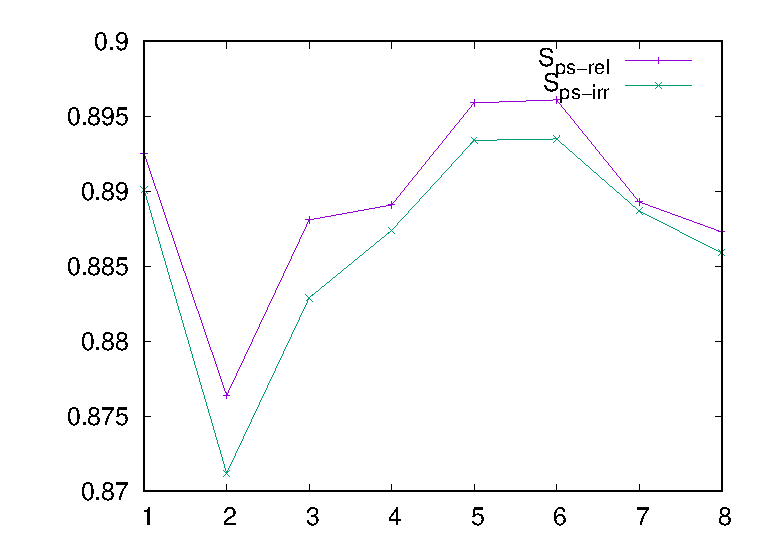
\includegraphics[scale=0.8]{314-1_scores.eps}}
    \caption{Оценки релевантности для модели}\label{fig:ep-scores}
\end{figure}